\chapter*{Abstract}

A szakdolgozatban fűtési rendszerek modell-prediktív szabályzásának lehetőségeit vizsgálom Matlab Simulinkben. %Szimulációval
Végighaladok az MPC tervezés lépésein, a tervezést és a validálást is szimulált szakaszmodellen végzem. A szakaszmodellt egy helyiség és annak fűtési rendszere alkotja, a fűtés hője a helyiségből külső homlokzaton távozik a környezet felé. Az állandósult állapotban szükséges fűtési teljesítményt képlettel számítom, ebből kapható a beavatkozó jel egy adott teljesítményigényhez. A hőkapacitásokat és hőátadási, hővezetési tényezőket Simscape modell tartalmazza%(\ref{table_heater_parameters}. és \ref{table_house_parameters}. táblázat)
, meghatározva a szakasz dinamikáját. Megvizsgálom az MPC predikciós horizontjának, költségfüggvényének illetve mintavételi idejének hatását a zárt szabályzási kör viselkedésére.  %tranziens viselkedését
%A szimulációhoz felállított modellhez számításokra is szükség van,
%Állandósult állapotra felírt képlet adja a szükséges fűtési teljesítményt

A tervezési lépéseket ezután valós, fizikai modellen is elvégzem, így látható lesz, hogy egy kész házra, vagy annak egy részére mennyi munkával jár a szabályzó beállítása. Ha a modellezésre, hangolásra fordított idő megtérül, azaz komfortnövekedéssel, illetve az üzemeltetési költségek csökkenésével jár, akkor a funkciókat akár az iContrALL okosház platformba is be lehet illeszteni.
%a módszer pénzbeli haszonnal is kecsegtet.

 % rendezzük a  \ref{eq_holeadas4}-t alpha-ra!

%a beavatkozók, a mérhető zavarások és a hibajel függvényében.
% kapom, ez méretezéshez és költségek számításához használható. 

\chapter{Bevezetés}

%Van egy ház
%
%Van egy fűtési rendszere
%
%Vannak szabályozható szelepek a szobákban
%
%Hogyan szabályozzuk?



Az Európai Unió energiafogyasztásának 40\%-át az épületek adják, a szén-dioxid-kibocsátás 36\%-a származik innen. Az energiahatékonyság növelése kiemelten fontos: a korszerűbb közintézmények, munkahelyek, lakóingatlanok olcsóbban fenntarthatók és javítják az emberek életminőségét. %A szmogot, a nagy szállópor-koncentrációt számos vidéki városban az elavult fűtési rendszerek okozzák. A szektorban hatalmas a potenciál

Az új építésű ingatlanoknak egyre szigorodó követelményeknek kell megfelelniük\footnote{2021-ben használatba vett ingatlanoknak már teljesíteniük kell a közel nulla energiaigényű épületekre vonatkozó szabályokat. Forrás: \\ e-epites.hu/e-tanusitas/az-energetikai-tanusitvany-kiallitasa-2016-tol \\ ec.europa.eu/energy/en/topics/energy-efficiency/buildings/nearly-zero-energy-buildings}.
%Európa / Magyarország energiafelhasználásának x százalékát az épületek adják, így a kibocsátás x százaléka is innen származik.
%A szmogot, a nagy szállópor-koncentrációt számos vidéki városban az elavult fűtési rendszerek okozzák.
%Ezek a tényezők életminőségünkre is kihatással vannak, ezért manapság számos újépítésű lakó- vagy irodaháznál figyelembe veszik az energiahatékonysági szempontokat.
A törvények előírják energetikai tanúsítvány készítését szerte az Unióban, ami ellenőrzi az épület megfelelőségét energetikai szempontból.
Azok a legújabb építésű, fenntartható irodaházak, amelyek WELL minősítést kapnak, az emberek egészségének és jó közérzetének fenntartását is segítik.

Ilyen fejlett technológiákat felvonultató épületekben nagy szerepet játszanak az épületgépészeti rendszerek (HVAC),
%\footnote{A HVAC (heating, ventilation, and air conditioning) rendszerek közé tartoznak a fűtési rendszerek is. Részletesen pl. a }
a 7/2006. TNM rendelet\cite{TNM2006} is megfogalmaz szabályokat és ajánlásokat ezzel kapcsolatban. Eszerint \say{új fűtési rendszer létesítésekor és meglévő fűtési rendszer korszerűsítésekor a helyiségenkénti hőmérséklet-szabályozást javasolt megvalósítani gazdaságossági számítás alapján}. 


%WELL tanúsítványt szerzett épületek ezen felül az emberek egészségének és jó közérzetének fenntartását is segítik.
%Itt viszont a fűtési, hűtési rendszerek szabályozására kevesebb hangsúly kerül, pedig ezekkel további megtakarítások érhetők el,

% lévén ezekre nehezebben írható elő általános kritérium.
% További megtakarítások illetve nagyobb komfortérzet érhető el a megfelelő szabályozással is. 


% Számos megtakarítási forma már régóta él a köztudatban, például a szigetelés, az ablakcsere. Alacsonyabb besorolás esetén az energetikai tanúsítványban is szerepel javaslat a korszerűsítésre. %Az ágazat úttörői az építészek, többnyire a szerkezetek tervezésénél veszik figyelembe a fenti szempontokat.
%Az üzemeltetési időszakra viszont kevesebb figyelem kerül, szerencsére manapság már a teljes élettartamra vetített költséget is figyelembe szokás venni.

%Sokszor ilyen esetben csak az épületszerkezetek kialakítására fordítanak kellő figyelmet - az előírások is erre vonatkoznak, az épületgépészeti rendszerek automatizálása viszont kevésbé elterjedt. Helyette sok helyen egyszerű termosztátokat használnak.% FORRÁS!!

%Irodaházakban van piaca bonyolultabb eljárásoknak.

%különben lakókörnyezetünkben
%A környezetvédelem és a költséghatékonyság 

Munkámban szeretnék megvalósítani egy helyiségenkénti hőmérséklet-szabályozást, ezen keresztül pedig megmutatni a különböző fűtési típusok viselkedését egy helyiségen belül.
\vspace{18pt}
%Kiindulási alapként az energetikai tanúsítványban szereplő paramétereket használom az épületek modellezésére

\pagebreak

A szabályzáshoz a klasszikus elképzelések szerint vagy ismerjük a szabályzott szakasz modelljét, vagy identifikálnunk kell azt, vagy fel kell írni rá a gerjesztés-válasz kapcsolatot, pl. átviteli függvényeket. 
%Mindhárom eset elképzelhető valamilyen szinten, egyes alrendszerek átvitelét esetleg könnyebben felírhatjuk, mások bizonytalan
%A felállított szakaszmodellben valamennyire mindhárom megjelenik. Új építésű lakásoknál a paraméterek többnyire ismertek (valamilyen pontossággal). Épületfizikai összefüggéseket felhasználva egyenleteket is fel lehet írni a hőfelvételre, hőleadásra. Ezen összefüggésekkel egyenértékű átviteli függvény is felírható, ha a rendszer bemeneteire gerjesztéseket adunk és mérjük a kimeneteket.  %\cite{AFRAM2014343}
%
A 2.-3. fejezetekben felállítok egy helyiség és a hozzátartozó fűtőtestek modelljét. Itt röviden foglalkozok méretezési kérdésekkel is, illetve ezeket felhasználom a modell megalkotásához. Publikációk, könyvek, adatlapok alapján validálom a felírt összefüggéseket, az ottani mérések adataiból kiindulva. (\cite[313.~o.]{Herz} - fűtőtest mérés, be kell helyettesíteni)


A törvény is javasolja helyi szabályzás kiépítését, illetve Csoknyai \cite[118.~o.]{Herz} is összegyűjtötte azokat a zavarásokat, amelyeket egy elosztottan működő rendszer jobban tud kezelni, mint egy központi szabályzás. Épületautomatikai rendszerek használatával tovább pontosíthatók ezek az információk, ezért a fűtésszabályzás integrációja az iContrALL okosotthon rendszerébe azért is előnyös, a fellépő zavarásokat (emberek jelenléte, napsütés, szél) mérhetővé teszi. Az integrációval további beavatkozók is használhatók, pl. redőny. %pl. infraszenzorokkal megmondható, hogy adott szobában tartózkodnak-e További 

% A hőátadási tényezők módosításával hűtés is szimulálható. Magasabb szintű szabályzással megadható a fűtő/hűtővíz hőmérséklete. Páratartalom mérése is megoldott, a szabályzás erre is kiterjeszthető.


A helyiség modelljére Simulinkben átviteli függvényt identifikálok (4. fejezet), erre megtervezem az MPC szabályzást (5. fejezet). A Matlab alapértelmezett paramétereit beállítom a fizikai korlátoknak megfelelően(...). Megvizsgálom a kapott teljesítményt.

Az MPC-nek rendkívül sok paraméterezési lehetősége van ---- (kazánok \cite[235.~o.]{Herz} szerint: kazánok hatásfoka, túlméretezése. )

Az MPC szabályozás gyakorlati kipróbálásához fizikai tesztrendszert állítunk fel, itt az MPC tervezési kérdésekre koncentrálok, átviteli függvény modellből.

%, melynek paramétereit energetikai tanúsítványból vehetjük. Ezzel egy közelítő modelljét megkapjuk a háznak, terepi mérések nélkül is lehetséges a szabályzás. A telepítés ideje lecsökkenthető, hiszen a hosszas kalibrálás elmarad.  A modellezéshez külön írom fel a helyiség és a fűtőtestek modelljét.%Természetesen bevethetők zárt körben végzett identifikációs módszerek, adaptív szabályzók is.

% az identifikációt potenciálisan elrontó hatások pedig nem jelentkeznek. Ugyanis megbízható identifikáció nagyon sok időt venne igénybe.\cite{THIEBLEMONT2017485}%\footnote{Thieblemont state of art weather fc MPC-ben szót ejt róla}
%(Adaptív szabályzást egyelőre nem használok.)





%Ehhez először áttekintettem a hőátadás lehetséges formáit és forrásait.
%Ezután fűtőtestek modelljét állítom fel.

%Helyi szabályzást valósítok meg, \cite[118.~o.]{Herz} szerint.




%\pagebreak

 %Arra jutottam, hogy ha a levegő hőmérsékletére szabályzok, akkor az abba beleszóló tényezőket veszem sorra:
%\begin{itemize}[noitemsep,topsep=0pt,parsep=0pt,partopsep=0pt]
%	\item konvektív hőátadás: a felszín közelében felmelegedett levegő áramlani kezd
%	\item radiatív hőátadás: sugárzással kibocsátott energia a környezetbe
%\end{itemize}

%\begin{figure}[h]
%	\centering
%	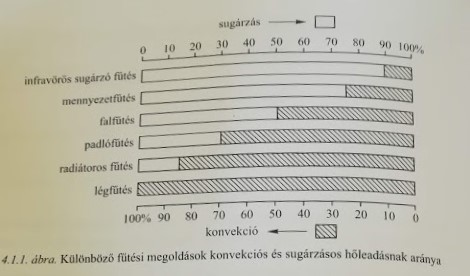
\includegraphics[width=8cm]{figures/konvrad}
%	\caption{Alacsony hőmérsékletű fűtés és magas hőmérsékletű hűtés c. könyv ábrája}
%		%\footnote{Jan Babiak, rehva Guidebook No.7}
%\end{figure}


%A levegő hőmérsékletére ezek a következőképp hatnak a leginkább:
%\begin{itemize}[noitemsep,topsep=0pt,parsep=0pt,partopsep=0pt]
%	\item a fűtőtestek konvektív és radiatív hőátadással is melegítik a környezetet
%	\item a radiatív energiát a tárgyak, falak nyelik el, amik ezáltal felmelegszenek (mintegy kapacitásként lesz egy hőtároló tömeg, ami a fűtés kikapcsolásával fenntartja a hőmérsékletet / lassítja a hűlést)
%	\item a fűtetlen falfelületek hűtik a szobát (külső hőmérséklet befolyása)
%\end{itemize}
%
%Így a kezdeti modellben azzal a feltételezéssel élek, hogy ezen kívül más hatás nem lép fel.
%
%A modellben feltételezem, hogy a fűtőtest felületi hőmérsékletével tudunk beavatkozni. A modellben paraméter a fűtőtestek hőátadási tényezője és felülete. Zavarásként (?) hat a külső hőmérséklet értéke, amit mérni is tudunk. Kimenet a belső hőmérséklet (térben konstansnak véve azt / átlagolva a szoba levegőjére)
%
%A modell felírásához a fűtőtest tulajdonságain kívül szükség van a szobában található levegő mennyiségére is. A zavarás hatását is fel kell írni, azaz hogy egy külső hőmérsékletváltozás hogyan jelenik meg a kimeneten. (Célszerű itt egy átviteli függvényt felírni először, szuperpozíciószerűen. A zavarás viszont nem a modell bemenetén és nem is a kimenetén hat.)

%A felírandó átviteli függvények:
%
%\begin{itemize}[noitemsep,topsep=0pt,parsep=0pt,partopsep=0pt]
%	\item levegő felmelegedése konstans külső hőmérsékletet feltételezve, fűtőtest egységugrással
%	\item levegő felmelegedése fűtés kikapcsolt állapota mellett, környezeti hőmérséklet ugrásával
%\end{itemize}
%
%Ezeket ráadtam a rendszerre és két bemenetű, egy kimenetű rendszerként identifikáltam.

%\pagebreak


%\subsubsection{Modellparaméterek}

%\subsection{-----}
%
%Fűtési típusok szerint:
%
%\begin{itemize}[noitemsep,topsep=0pt,parsep=0pt,partopsep=0pt]
%	\item radiátoros fűtés hőátvitele
%	\item padlófűtés hőátvitele
%\end{itemize}
%
%A fentiekre különböző értékű lesz a 
%
%\begin{itemize}[noitemsep,topsep=0pt,parsep=0pt,partopsep=0pt]
%	\item hőátadási tényező
%	\item hőtároló tömeg
%	\item költségfüggvény?
%	\item előremenő vízhőmérséklet és ezzel a leadott teljesítmény maximumértéke
%\end{itemize}
%
%ami így eltérő ház-modelleket fog eredményezni.
%











\pagebreak